\documentclass{article}
\usepackage[utf8]{inputenc}
\usepackage[legalpaper, portrait, margin=0.8in]{geometry}
\usepackage{amssymb}
\usepackage{hyperref}
\usepackage{graphicx}

\hypersetup{
    urlcolor=cyan, 
    linkcolor=blue
}

\title{Machine Problem 1: Cache Design, Memory Hierarchy Design}
\author{Kobee Raveendran}
\date{October 28, 2021}

\begin{document}
    \begin{titlepage}

        \maketitle
        \null  % Empty line
        \nointerlineskip  % No skip for prev line
        \vfill
        \let\snewpage \newpage
        \let\newpage \relax
        \centering
        {\large \textbf{Honor Pledge: ``I have neither given nor received unauthorized aid on this test or assignment.''}}
        
        \centering {\large Student's electronic signature: \underline{ Kobee Raveendran }}

        \vspace{6cm}
        {\large \textbf{University of Central Florida}}
        
        \vspace{1cm}

        {\large \textbf{Department of Computer Science}}

        \vspace{1cm}

        {\large \textbf{CDA5106: Advanced Computer Architecture}}

        \vspace{1cm}

        {\large \textbf{Fall 2021}}
        \let \newpage \snewpage
        \vfill 
        \break % page break
        
    \end{titlepage}

    \section{L1 Cache Exploration: Size and Associativity}

    \begin{center}
        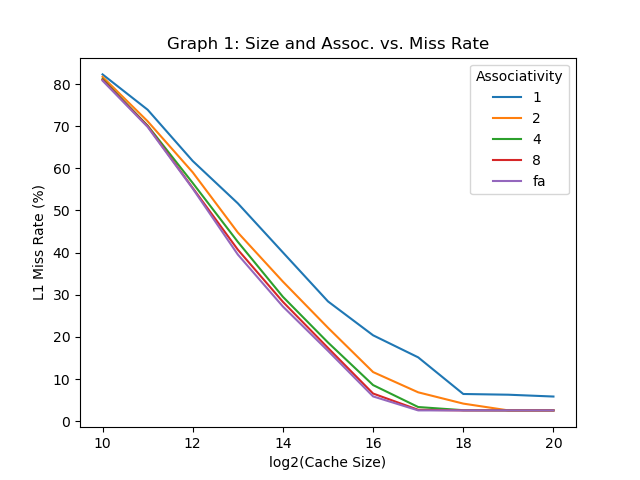
\includegraphics[width=\textwidth]{../graph_logs/graph1.png}
    \end{center}

    For this experiment, L1 size varies between $2^{10}$B and $2^{20}$B (1kB and 1MB, respectively), while 
    associativity varies between 1-8, and additionally fully-associative (which is $\frac{size}{blocksize}$). 

    Several trends appear in the graph, exposing the relationship between cache size, associativity, and miss rate:
    
    \begin{enumerate}
        \item As cache size increases, L1 miss rate decreases universally (regardless of associativity).
        \item Additionally, increasing cache associativity also decreases L1 miss rate, though not as drastically 
        as a cache size increase would (note that, at any fixed cache size, the variance in miss rate between the different associativity 
        values is noticeable, but still very slight at times).
        \item Increasing associativity yields diminishing returns; note that, as cache size increases, the difference in 
        associativity between assoc-8 and assoc-FA will increase. However, on the right half of the graph, it's easy to 
        see that the difference in miss rate between an 8-way set-associative cache and a fully-associative one is minimal.
    \end{enumerate}

    Miss rate estimations:

    \begin{itemize}
        \item \textbf{compulsory misses:} These are inevitable misses, resulting from having to fetch blocks from 
        memory the first time they're needed in the cache. I estimate an average of 4\% of all misses are compulsory, 
        based on the performance of a fully-associative cache (which has the lowest conflict miss rate), since these are misses that would occur even in a ``perfect'' and 
        infinitely-sized cache with full associativity and LRU replacement. I arrived at about ~4\% because that seems 
        to be the miss rate that the cache would converge to as cache size and associativity tended toward infinity, 
        indicating that a miss rate of 4\% is a lower bound (which makes sense because these misses are inevitable).

        \item \textbf{conflict misses:} These are caused by collisions or conflicts in which there are more blocks to 
        be placed in a set than the set can hold (thus bottlenecked by cache associativity). Based on this, it makes sense 
        that a fully-associative cache with LRU replacement would have a low (if not zero) conflict miss rate, while a 1-way 
        set-associative cache would have the highest conflict miss rate. Below are some rough guesses based on the graph 
        and intuition:

        \begin{itemize}
            \item \textbf{1-way:} 
            \item \textbf{2-way:} 
            \item \textbf{4-way:} 
            \item \textbf{8-way:} 
            \item \textbf{fully-associative:} 0\%
        \end{itemize}

    \end{itemize}

    \newpage

    \section{L1 Cache Exploration: Size and Associativity vs. AAT}

    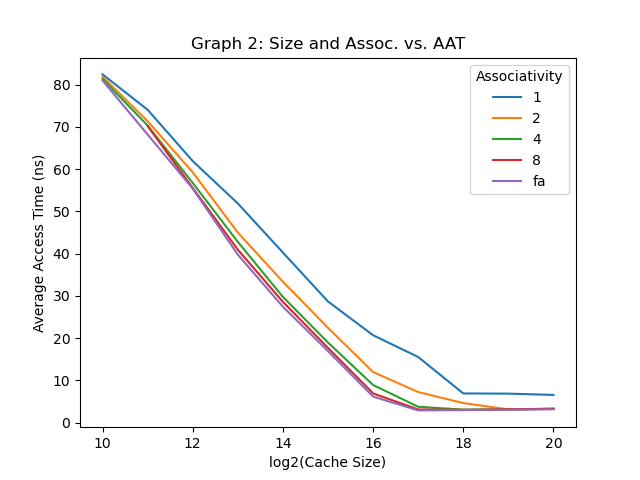
\includegraphics[width=\textwidth]{../graph_logs/graph2.png}

    In this experiment, L1 cache size and associativity vary in the same ranges as described in experiment 1, but here 
    average access time (AAT) is measured instead of L1 miss rate (some points excluded, like $x = 10$ with assoc. = 
    8, as such points where not included in the CACTI table). Note the similarity in pattern/trend in this graph 
    compared to the graph in experiment 1.

    Based on the graph's trends, the best possible cache configuration to choose given the parameters plotted (assuming 
    others, like block size, staying fixed), would be the fully-associative cache with a size between $2^{17}$ and 
    $2^{20}$ bytes (depending on whether the AAT starts increasing again, which is hard to tell from the plot alone). 
    However, an 8-way set associative cache (with a size lying in that same interval) is almost as good and would serve as a decent alternative candidate given 
    the weaknesses of a fully-associative cache.

    \newpage

    \section{Replacement Policy Study}

    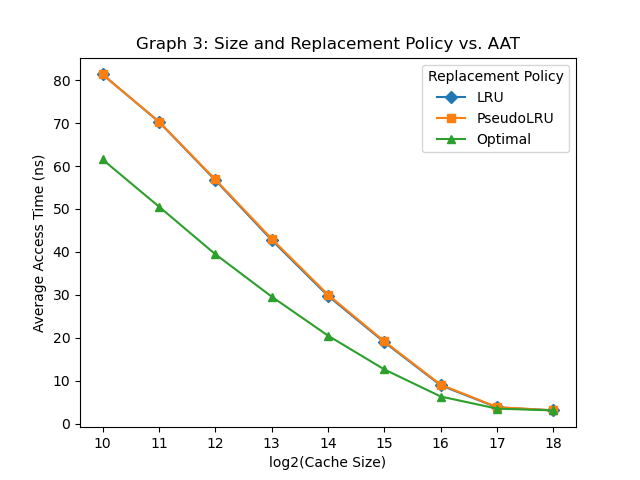
\includegraphics[width=\textwidth]{../graph_logs/graph3.png}

    In this experiment, L1 cache size varies between $2^{10}$B and $2^{18}$B (1kB and 256kB, respectively), while 
    the replacement policy varies between LRU, PseudoLRU, and optimal.

    Of course, the best-performing cache is one with the largest size (256kB) that uses the optimal replacement policy. 
    This makes sense because this policy guarantees the replacement of the block that will not be needed for the longest 
    period of time (or never again), so less time is spent re-fetching blocks from memory in case an evicted block 
    needed to be in the cache again soon after its eviction. However, since optimal replacement is impossible to implement 
    in practice, I'd also like to compare LRU and PseudoLRU, which are both practical.

    While they appear to yield exactly equal performance, when viewing my simulation stats, I did notice a slightly-worse 
    performance in PseudoLRU (to view my simulation run logs, run \texttt{simulation\_manager.py} in 
    \href{https://github.com/kobeeraveendran/cda5106/tree/master/hw/MachineProblem1_Fall2021/cachesim}
    {my repository}). However, considering the fact that LRU is more memory-efficient in practice, and can 
    still approximate LRU almost unnoticeably-closely, it could be a better candidate between the two.

    \newpage

    \section{Inclusion Property Study}
    
    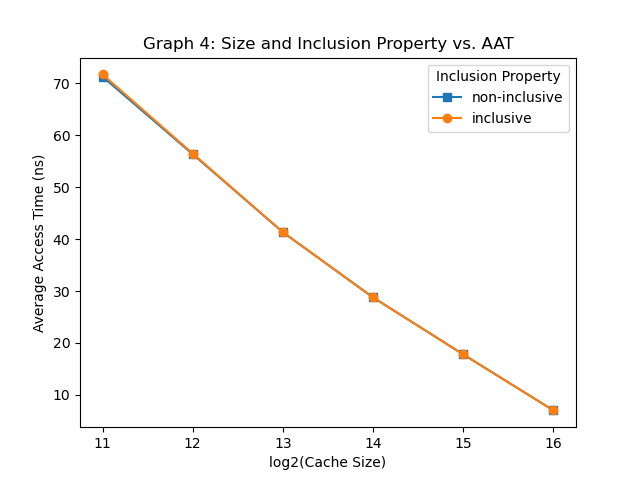
\includegraphics[width=\textwidth]{../graph_logs/graph4.png}

    In this experiment, cache size varies between $2^{11}$B and $2^{16}$B (2kB and 64kB, respectively), while 
    the inclusion property is either non-inclusive or inclusive.

    Interestingly enough, the inclusivity of the caches does not seem to matter much in this experiment (between a cache 
    that is inclusive and one that is non-inclusive). Only in the smallest cache size does the non-inclusive cache 
    yield a lower AAT, but afterwards, they both seem to exactly match (unnoticeably small differences, if any).

    That said, I do not imagine this same trend would hold if they were both compared to an exclusive outer cache (not 
    tested here). That is because there will be less cache coherency (since each cache level has unique items), but 
    better memory utilization (no redundancy) and \textit{potentially} worse (higher) access time. This last point will 
    be due to the fact that inclusive caches can eliminate the need to search entire cache levels (i.e. if a block is not 
    found in the outermost cache, we do not need to search in any of the inner caches), while exclusive and non-inclusive 
    caches do not necessarily have this luxury.

\end{document}

